% !TeX spellcheck = it_IT
\section{Mobile Network}

\subsection{Introduzione alle reti mobili}

\paragraph{Pre-Cellulare:} Prima degli anni '80 esistenza un servizio di telefonia mobile con trasmettitori e ricevitori ad elevata potenza, con 25 canali e 80km di raggio di copertura. Capacità insufficiente per fornire un servizio di telefonia (voce) comparabile con i servizi di telefonia fissi.\\

L'idea dietro la rete cellulare invece è usare \textbf{molteplici trasmettitori} con una potenza "bassa", minore di 100W. Meno potenza, meno raggio di copertura: l'area viene divisa in celle (da qui "cellulare"), ognuna con una propria antenna (o più).\\

Ogni cella è servita da una \textbf{Base Station (BS)}:
\begin{itemize}
	\item Trasmettitore
	\item Ricevitore
	\item Unità di controllo
\end{itemize}
Può operare in licensed/unlicensed spectrum.\\

La progressione è:
\begin{itemize}
	\item 1980 \textbf{1G Advanced Mobile Phone Service (AMPS)}: Voce analogica in mobilità
	\item 1990 \textbf{2G Global System for Mobile Communication (GSM)}: Voce digitale (compressa, \dots), prima rete globale
	\item 2000 \textbf{3G Universal Mobile Telecommunications System (UMTS)}: Introduce i servizi internet
	\item 2010 \textbf{4G Long Term Evolution (LTE)}: convergenza IP e aumento delle prestazioni
	\item 2020 \textbf{5G}: Networks softwarization \& virtualization, slicing \& bassa latenza
	\item 2030 \textbf{6G}: Network intelligence (AI all'interno della rete, ottimizzazione secondo AI)
\end{itemize}

Gli standard della rete cellulare si possono vedere su \href{https://www.3gpp.org/specifications-technologies/releases}{\texttt{Third Generation Partnership Project (3GPP)}}. Sono tutte le release su cui si basano i rilasci commerciali.\\

\paragraph{Base Station BS:} Un esempio di BS può essere
\begin{center}
	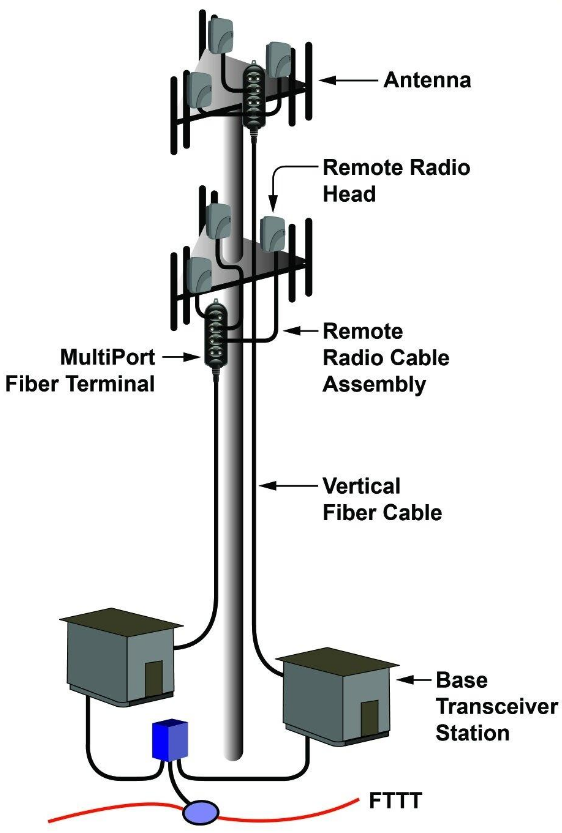
\includegraphics[width=0.4\linewidth]{img/mobile/1BS}
\end{center}

Le componenti sono:
\begin{itemize}
	\item \textbf{Antenna}: trasmette e riceve onde radio
	\item \textbf{Remote radio head}: riceve i segnali analogici e li converte in digitale e viceversa; vicino all'antenna per ridurre la perdita di segnale nei cavi
	\item \textbf{Remote radio cable assembly}: gruppo di cavi che fornisce alimentazione e/o collegamento dati tra la stazione base e i Remote Radio Heads
	\item \textbf{MultiPort Fiber Terminal}: punto di terminazione o distribuzione in cui la fibra ottica in entrata viene divisa o collegata a più uscite per servire le diverse RRH. In pratica, funge da "scatola di giunzione" per organizzare e connettere i vari cavi in fibra destinati ai moduli radio remoti
	\item \textbf{Base Transceiver Station (BTS)}:L'elemento principale dell'infrastruttura della rete mobile, gestisce il traffico dati e vocale, coordina i protocolli radio, si interfaccia con la rete di trasporto verso il core network dell'operatore e invia i segnali digitali agli RRH. Al suo interno si trova l'elettronica di baseband (elaborazione del segnale, modulazione/demodulazione, protocolli) e vari componenti di controllo
\end{itemize}

\subsection{Organizzazione Geometrica delle Celle}

Bisogna capire come disporre le celle. I requisiti sono:
\begin{itemize}
	\item coprire "bene" l'area
	\item avere una disposizione uniforme
\end{itemize}

Una buona disposizione usa celle esagonali per una copertura e disposizione uniforme. Ovviamente si tratta della disposizione ideale, nella realtà ci sono dei vincoli, di posizionamento e diffusione del segnale.\\

\paragraph{Riuso delle frequenze:} Si ha il problema di avere celle vicine con la stessa banda di frequenza: dispositivi sui bordi ricevono dati da entrambe le celle. \\

La prima soluzione è usare \textbf{frequenze diverse tra celle vicine}, ma servono più bande (licensed spectrum, costa e ne uso solo una parte per volta). 2G opera in questo modo.\\

Un'altra soluzione, per non "sprecare" banda, è usare la stessa frequenza e \textbf{tecniche di codifica} per evitare le interferenze tra celle vicine (\textbf{CDMA}).\\

L'ultima soluzione è:
\begin{itemize}
	\item al \textbf{centro} di ogni cella usare l'\textbf{intera ban}da disponibile (tranne un pezzo), per gli utenti interni
	\item al \textbf{bordo}, \textbf{celle vicine} hanno \textbf{frequenze diverse}
\end{itemize}

Questo permette bandwidth maggiore per utenti interni ma richiede un sofisticato controllo di potenza e coordinamento tra BS (4G e 5G). Bisogna posizionare all'interno della cella i dispositivi in maniera abbastanza precisa per stabilire che frequenze utilizzare. \\

%fino s16
%End L15

\newpage

\subsubsection{Aumento della capacità per migliorare la scalabilità}
 
Uno degli obiettivi fondamentali delle reti cellulari è servire sempre più utenti utilizzando lo spettro disponibile (costo elevato), evitando di utilizzare ed installare troppe BS. La rete cellulare è formata da celle, e una BS può contenere più celle.\\ 

Una gestione dinamica delle frequenze tra celle vicine permetterebbe il prestito di frequenze, con i relativi costi di sincronizzazione.\\

Si possono aumentare le celle, suddividendole e rendendole più dense in aree con più elevato traffico, ma più celle ci sono più è frequente il cambio di cella (handoff/handover), con il relativo traffico di controllo.\\

\paragraph{Cell sectoring:} Una BS può avere diverse antenne direzionali (al posto di una omnidirezionale) che permettono di creare diverse celle
\begin{center}
	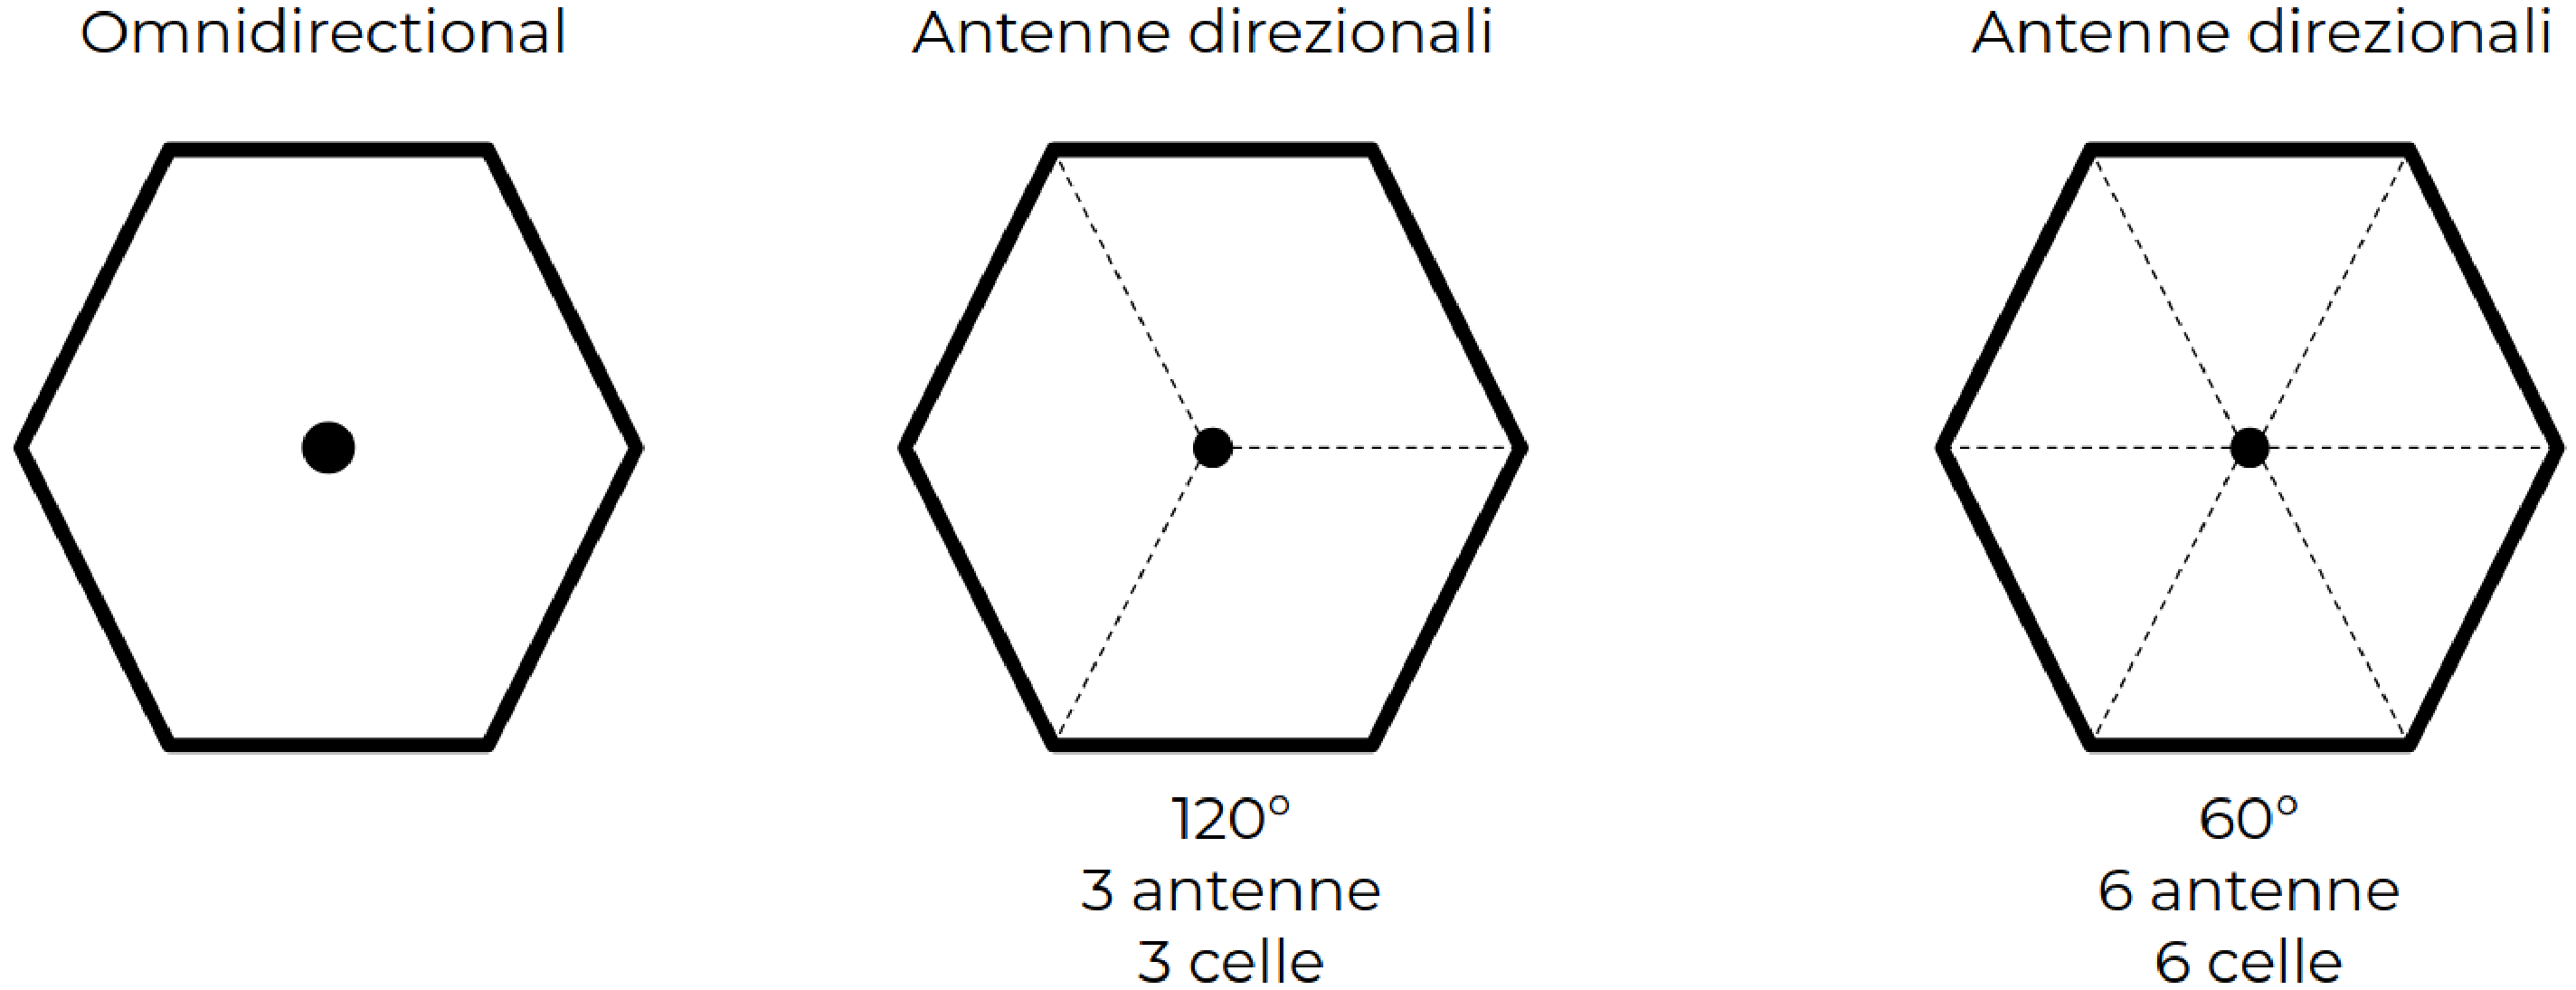
\includegraphics[width=0.8\linewidth]{img/mobile/sectoring}
\end{center}

Sono effettivamente celle diverse, con i relativi problemi di bordo e handover, ma restringere la cella permette di migliorare il data rate. Dare una direzionalità di gain molto alta permette di ridurre il path loss (\textbf{Beamforming}).\\

\newpage

\subsection{Architettura}

L'architettura di una rete cellulare si divide in grosse macro aree: 
\begin{itemize}
	\item \textbf{Radio Acces network RAN}: la parte di stazioni e collegamento radio che forniscono collegamento ai dispositivi mobili
	\item \textbf{Core Network}: la parte centrale responsabile della gestione e del controllo della comunicazione tra utenti e servizi esterni
\end{itemize}
\begin{center}
	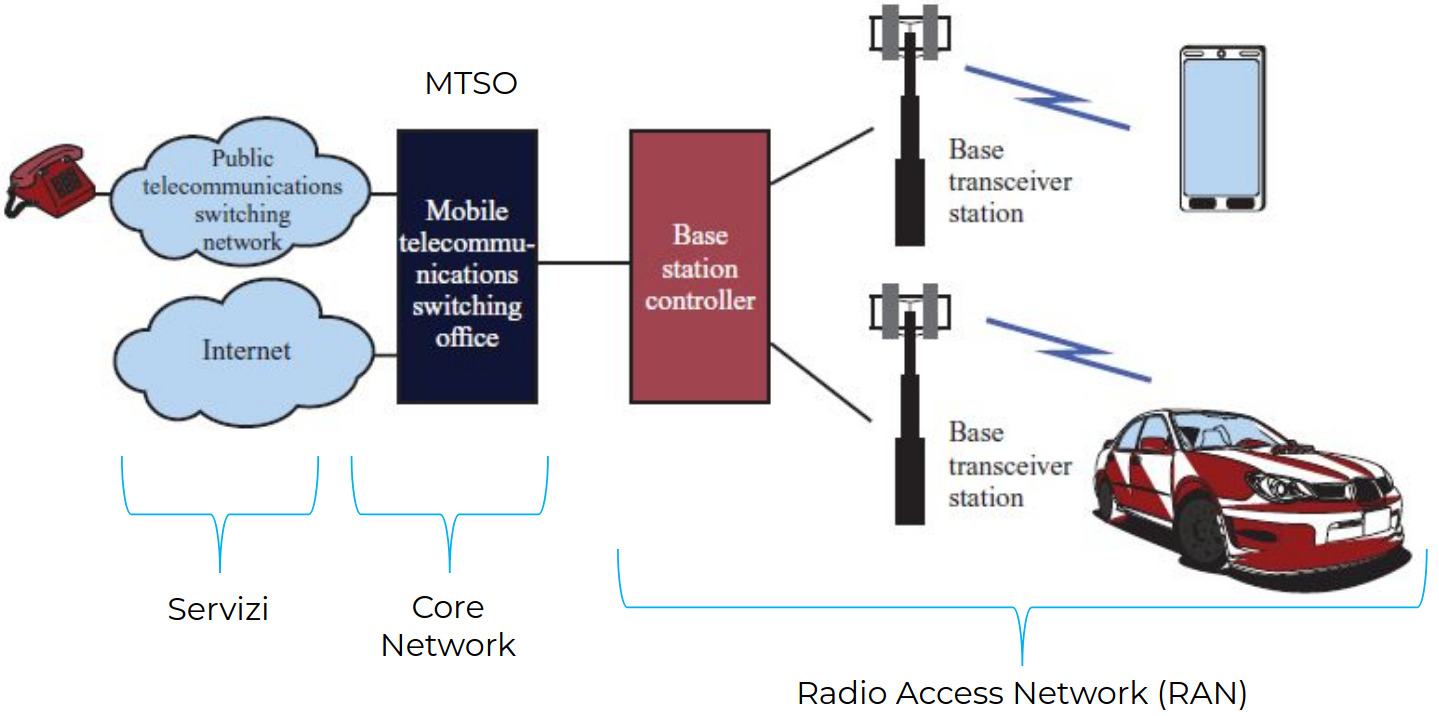
\includegraphics[width=0.8\linewidth]{img/mobile/archop}
\end{center}
Tutto il core network è rete fissa, fino alle antenne, per poi essere wireless. \\
%Boh, compl
Tutte le operazioni delle rete cellulare sono automatiche e non richiedono alcun intervento da parte dell'utente. Si ha una separazione netta tra quelli che sono i canali di controllo, fisici o virtuali. \\

Esistono \textbf{2 tipi di canali} che trasportano 2 tipologie di traffico:
\begin{itemize}
	\item \textbf{Canali di controllo}: trasportano tutte le informazioni per la gestione delle operazioni, \textbf{Control Plane} (es. handoff, autenticazione, \dots)
	\item \textbf{Canali di traffico}: trasportano voce e dati (traffico dei servizi offerti all'utente), \textbf{Data Plane}
\end{itemize}
Si ha una divisione Control/Data plane netta ed esplicita.\\

\newpage

\subsection{Operazioni}

\paragraph{Inizializzazione:} Ci sono diverse funzionalità. Si ha una fase di inizializzazione che serve a capire i segnali che vengono ricevuti, il dispositivo utente monitora i segnali delle celle per identificare quella migliore. Periodicamente ogni BS invia dei \textbf{pilot} che permettono al dispositivo di determinare la qualità del segnale di quella cella.\\

Quando un dispositivo vuole iniziare una comunicazione con la rete cellulare:
\begin{enumerate}
	\item \textbf{Disponibilità di canali radio con BS}: ascolta le trasmissioni broadcast delle BS per individuare quale cella ha segnale sufficiente, quali canali radio sono liberi e quali parametri di accesso usare
	\item \textbf{Traffico di controllo per iniziare la comunicazione con MTSO}: viene inoltrata la richiesta di comunicazione, fino al MTSO, che si occupa di autenticare l'utente, verificare permessi e risorse, decidere se e come procedere (Core network)
	\item \textbf{Creazione dei "collegamenti" su data plane}: se la fase di controllo va a buon fine, vengono allocati i canali fisici e logici necessari per il traffico dati, il dispositivo potrà cominciare a scambiare dati liberamente
\end{enumerate}

\paragraph{Paging:} L'operazione di pagine è il "cercare" il dispositivo, perché c'è \textit{qualcosa} che deve raggiungerlo. I device non sono sempre attivi nella rete cellulare, quindi potrebbe essere necessario cercarli. Il dispositivo si può muovere in completa libertà, è \textbf{compito della rete} "ritrovare" la posizione quando necessario.\\

MTSO non è sempre a conoscenza della posizione del dispositivo (ovvero la cella a cui è associato), il dispositivo può essere in idle mode (senza una connessione attiva). MTSO quindi contatta le BS delle celle per "trovare" il dispositivo.\\

\newpage

\paragraph{Chiamata accettata:} La chiamata (in realtà i dati, si parla in generale) passa \textbf{sempre} attraverso il core network:
\begin{itemize}
	\item Il dispositivo destinatario accetta la chiamata
	\item MTSO crea un circuito (fino a 3G, da 4G VoIP)
	\item le BS impostano i canali radio data plane
\end{itemize}

Durante una chiamata I due dispositivi si scambiano informazioni attraverso le BS a cui sono collegate e MTSO. In realtà, oltre a up e down link, può esistere il side link: un meccanismo che permette di bypassare BS e (in parte) core network per la comunicazione; nasce per scenari Device-to-Device D2D e Vehicle-to-Everything V2X.\\

\paragraph{Handoff:} I dispositivi possono muoversi al di fuori del raggio della cella nella quale hanno iniziato la comunicazione. Serve collegarsi ad un'altra cella; le fasi sono:
\begin{enumerate}
	\item Decisione di nuova associazione
	\item Gestione nuova associazione
	\item Riconfigurazione percorsi di comunicazione
\end{enumerate}

Il tutto deve avvenire in maniera \textbf{automatica} e \textbf{senza interruzione della comunicazione} (entro certi limiti della tecnologia, ad esempio meno di 200km/h).\\

\newpage

\subsection{Ambiente}

Il contesto nel quale la rete cellulare opera è molto più dinamico e imprevedibile degli altri scenari wireless. Contesti \textbf{molto eterogenei} e molto complessi. \\

La \textbf{potenza del segnale} deve essere: 
\begin{itemize}
	\item sufficiente per offrire un servizio di buona qualità
	\item non troppo per non creare interferenza
	\item molto variabile per via degli ostacoli
\end{itemize}

Il \textbf{fading} (attenuazione del segnale) dipende anche da frequenza e tipo di ambiente.\\

\subsubsection{Deployment}

Gli operatori di rete mobile pianificano con molta attenzione l'installazione delle BS al fine di ottimizzare la rete. Operazione chiamata Network Planning. Questo include:
\begin{itemize}
	\item Posizionamento delle BS
	\item Dimensionamento delle BS
	\item Rete di trasporto verso MTSO
	\item Bande da utilizzare (frequenze più basse maggiore copertura, bandwidth limitata, frequenze più alte maggiore bandwidth, minore penetrazione ostacoli)
\end{itemize}

\newpage

\subsection{Handoff/Handover}

Uno degli aspetti più rilevanti è la \textbf{gestione dell'handover}, ovvero il cambio da una cella all'altra. La procedura può essere decisa in due modi:
\begin{itemize}
	\item \textbf{solo dalla rete}: basata sulla misurazione del segnale ricevuto dal dispositivo (uplink)
	\item \textbf{dispositivo coinvolto nella decisione}: fornisce un feedback sul segnale percepito (downlink)
\end{itemize}
Diverse metriche vengono monitorate dalle BS per prendere una decisione, ma il parametro principale per la decisione è la potenza del segnale ricevuta a livello di BS (e dal dispositivo coinvolto).\\

Il metodo più semplice è guardare \textbf{solo la potenza relativa}: l'associazione viene fatta alla BS che ha il migliore segnale. Ma l'handover è una procedura costosa e il segnale potrebbe fluttuare (ad esempio sui bordi della cella), portando all'effetto ping pong, ovvero un cambio continuo tra le BS. Questo può essere parzialmente risolto tenendo sul device uno storico delle BS a cui si è collegato, evitando di ri-collegarsi a BS da cui è stato fatto handover di recente.\\

Il primo miglioramento può essere \textbf{introdurre una soglia}: se il segnale è abbastanza buono (oltre una soglia), perché cambiare? L'handover ora viene effettuato solo nel caso il segnale sia peggiore di un'altra BS ma deve anche essere sotto una certa soglia. Si ha il problema di definire queste soglie, in quanto dipendono da diverse condizioni di contesto.\\

\newpage

Un altro miglioramento è aggiungere \textbf{isteresi}: si tiene un margine, per far partire l'handover deve esserci una differenza significativa di potenza. 
\begin{center}
	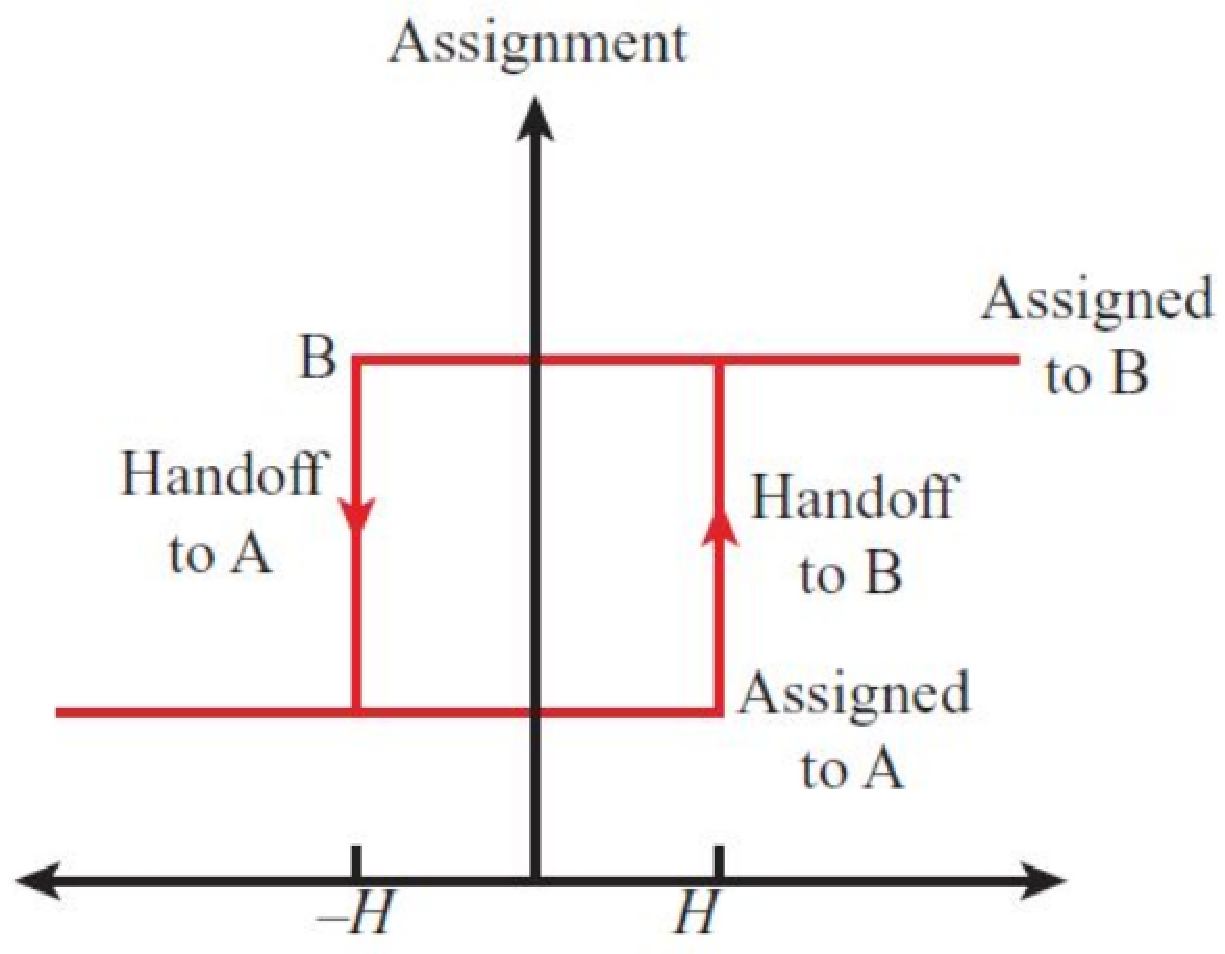
\includegraphics[width=0.55\linewidth]{img/mobile/isteresi}
\end{center}

Risolve il Ping-Pong ma rimane il problema che il segnale della prima BS può essere ancora "abbastanza buono". Si possono \textbf{combinare le idee}, per determinare l'handover si usano 
\begin{itemize}
	\item \textbf{potenza relativa}: deve essere abbastanza grande
	\item \textbf{soglia}: il segnale deve essere abbastanza "brutto"
	\item \textbf{isteresi}: la differenza deve essere significativa
\end{itemize}

\paragraph{Hard vs Soft Handoff:}
\begin{itemize}
	\item \textbf{Hard handoff}:
	\begin{itemize}
		\item il dispositivo è associato ad una sola BS alla volta
		\item cambio immediato di frequenza per agganciarsi alla BS vicina
		\item protocolli di handoff vicini
	\end{itemize}
	
	\item \textbf{Soft handoff}
	\begin{itemize}
		\item il dispositivo mantiene la connettività con entrambe le BS
		\item il rilascio di una BS quando il segnale è chiaramente dominante
		\item richiede più risorse in quanto il dispositivo è allocato più volte
	\end{itemize}
\end{itemize}

\newpage

\subsection{Duplex}
Per la gestione del duplex ci sono 2 modalità:
\begin{itemize}
	\item \textbf{Frequency Division Duplex FDD}: utilizzo di frequenze diverse per uplink e downlink; minore delay, maggiori risorse richieste
	\item \textbf{Time Division Duplex TDD}: una sola frequenza sia per uplink che downlink, maggiore ritardo perché bisogna aspettare
\end{itemize}

\subsection{GSM Mobile Station (MS)}

Si intende un dispositivo, cambia un po' nome attraverso alle generazioni ma sempre terminale finale si intende. In generale la struttura è
\begin{center}
	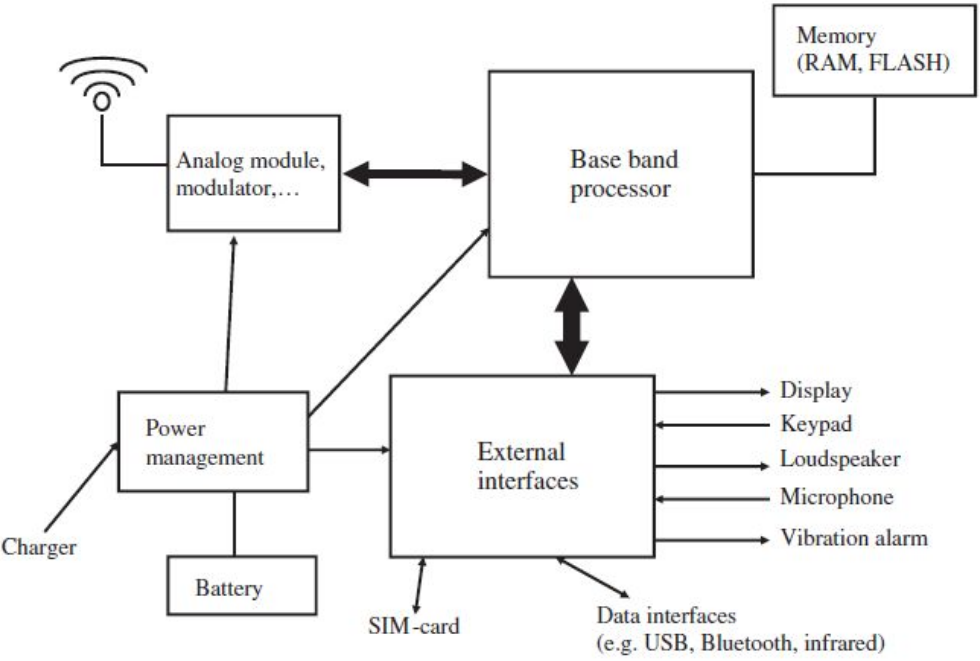
\includegraphics[width=0.65\linewidth]{img/mobile/ms1}
\end{center}

Ogni dispositivo (solo terminale mobile) possiede un identificativo unico detto \textbf{Internetional Mobile Equipment Identiity IMEI} (15 cifre). Hanno struttura
\begin{center}
	%\renewcommand{\arraystretch}{1.4}
	\begin{tabular}{| >{\centering\arraybackslash}m{3cm} | >{\centering\arraybackslash}m{2cm} | >{\centering\arraybackslash}m{3cm} | >{\centering\arraybackslash}m{2cm} |}
		\hline
		\textbf{TAC (6)} & \textbf{FAC (2)} & \textbf{SN (6)} & \textbf{Check digit (1)} \\
		\hline
		Type Approval Code, Codice del costruttore & 
		Final Assembly Code, Luogo costruzione & 
		Numero seriale & 
		Numero di controllo di validità del codice \\
		\hline
	\end{tabular}
\end{center}

Identificano a livello mondiale ogni dispositivo mobile.\\

\newpage

\subsubsection{SIM Card}

La SIM contiene informazioni per \textbf{identificare l'utente} (abbonato) e la chiave segreta per autenticazione e generazione chiavi di cifratura, reti preferite e proibite, PIN, PUK, ultime location, ecc.\\

Si hanno diversi formati, di diverse dimensioni, fino a Embedded SIM (eSIM), un chip programmabile all'interno del dispositivo.\\

Ha un \textbf{International Mobile Subscriber Identity IMSI} (diverso dal numero di telefono), il quale identifica una specifica SIM card (max 15 cifre).\\

Il numero di telefono viene chiamato \textbf{Mobile Subscriber Integrated Service Digital Number MSISDN}. Struttura:
\begin{center}
	\begin{tabular}{| >{\centering\arraybackslash}m{2cm} | >{\centering\arraybackslash}m{2cm} | >{\centering\arraybackslash}m{4cm} | }
		\hline
		\textbf{CC} & \textbf{NDC} & \textbf{Numero} \\
		\hline
		Country CODE & Network Destination Code & Numero utente \\
		\hline
		+39 & 123  & 1234567 \\
		\hline
	\end{tabular}
\end{center}

Si può avere l'associazione 1:1 tra SIM e numero di telefono, oppure un'associazione 1:N. Funzionalità per la portabilità del numero telefonico. \\

Il campo NDC, dopo l'introduzione della portabilità del numero, non ha più senso, non rappresenta più l'operatore.\\

%%%%%%%%%%%%%%%%%%%%%%%%%%%%%%%%%%%%%%%%%%%%%
% STORY TIME %
%%%%%%%%%%%%%%%%%%%%%%%%%%%%%%%%%%%%%%%%%%%%%

\newpage

\subsection{Story Time: Prima del 4G}

\subsubsection{Global System for Mobile Communications GSM}

Standard sviluppato all'inizio degli anni '90. Inizialmente la trasmissione dati era di tipo Circuit Switched (principalmente voce, ogni chiamata aveva una linea dedicata).  Riutilizzava tecnologie preesistenti, principalmente per la telefonia fissa, adattate pe rla rete mobile. All'inizio la trasmissione era analogica, dalla seconda metà degli anni '80 la voce comincia ad essere digitalizzata.\\

Dalle prime versioni di GSM circuit-switched si è progressivamente passati a soluzioni basate su Virtual Circuit Switching over IP (da commutazione di circuito a soluzioni IP-based). Si crea un "circuito virtuale" con una connessione logica temporanea su una rate IP. Risorse allocate in modo bidirezionale per tutta la durata del servizio.\\


Viene standardizzato dall'ETSI (European Telecommunication Standard Institute), prima a livello europeo, poi mondiale. Si tratta della prima volta in cui sono presenti standard comuni. Da UMTS in poi la standardizzazione è affidata a 3GPP.\\

Come si trasmette? Interfaccia radio tra device e base station è denominata Um ("U mobile", da ISDN). Usa Frequency Division Duplex (FDD), 2 bande attorno ai $900MHz$, $25MHz$ ognuna. Ogni banda è divisa in 125 canali da $200kHz$. \\

Una singola cella può avere estensione fino 35km (teoricamente, molto meno nella pratica). Suddivisione in celle e settori più piccoli permette di aumentare la capacità. Si ha una pianificazione del riuso delle frequenze in base alla posizione delle celle.\\

GSM implementa il multiple access usando due tecniche: 
\begin{enumerate}
	\item FDMA (divisione in frequenza): Divide lo spettro disponibile in canali da $200 kHz$, con 125 canali per direzione (Uplink e Downlink, $25MHz$ ciascuno). Tuttavia, non tutti i canali possono essere usati in ogni cella per evitare interferenze tra celle vicine
	\item TDMA (divisione temporale): ogni canale in frequenza può essere diviso in 8 slot temporali, permettendo l'accesso a 8 dispositivi tramite turni di trasmissione
\end{enumerate}

La trasmissione duplex non è possibile, i dispositivi devono alternare la trasmissione e la ricezione, richiede tempo. \\

\subsubsection{General Packet Radio Service GPRS \& Enhanced Datarates for GSM Evolution EDGE}

La rete GSM è perfetta per trasportare traffico voce: 
\begin{itemize}
	\item bit rate costante
	\item risorse pre-allocate e riservate (Time slot TDM diverso per ogni utente)
	\item delay costante (time slot TDM)
	\item No overhead di informazioni per segnalazione
	\item Tariffazione a durata (pago minuti/scatti)
\end{itemize}
ma anche per trasportare SMS:
\begin{itemize}
	\item Servizio delay-tolerant su canale di segnalazione
	\item Contenuto testuale semplice
	\item Tariffazione per SMS
\end{itemize}

Ma la rete GSM è idonea per offrire un servizio dati internet? 
\begin{itemize}
	\item Il traffico dati Internet ha un data rate variabile e l'interazione è intermittente e a burst
	\item Circuit-switched non è ottimale:
	\begin{enumerate}
		\item Le risorse pre-allocate sono inutilizzate per molto tempo
		\item Allocazione fissa non compatibile con traffico dati Internet
		\item Le risorse non utilizzate sono sprecate e non utilizzabili da altri utenti
	\end{enumerate}
	\item La tariffazione a durata non ha molto senso con dati Internet
\end{itemize}

GPRS è una rete a pacchetto (packet switched) realizzata come overlay (RAN) e aggiunta (Core) della rete GSM. Cerca di mantenere fissa la parte di RAN e Core per adattarla all'uso di internet. Permette: 
\begin{itemize}
	\item Data rate per utente di $20kbps$ ($270kbps$ EDGE)
	\item Tariffazione a volume di traffico
	\item Rilascio degli slot in idle (per natura burst del traffico)
	\item "Ridotto" tempo di connessione ad internet (da 20s GSM a 5s GPRS)
	\item La connessione (logica) non viene rilasciata, vengono rilasciati solo i time-slot radio; libera le risorse radio, mantiene l'IP associato
	\item La connessione (logica) è indipendente dalla connessione fisica, la mobilità o la perdita di copertura non interrompe la connessione
\end{itemize}

\subsubsection{GPRS Tunneling Protocol GTP}

Il GTP risolve il problema della mobilità per IP: dove invio i pacchetti se il dispositivo continua a muoversi? Non è possibile aggiornare le tabelle di routing ad ogni cambio della rete.\\
La connessione logica tra MS e GGSN è identificata da una sessione del protocollo Packet Data Protocol (PDP). MS è libero di muoversi all'interno della rete e possiede un proprio IP unico all'interno della rete (DHCP/NAT) e mantenuto per tutta la durata della sessione.\\

La soluzione è creare tunnel virtuali tra nodi della rete mobile, incapsulare il pacchetto, fornire un Tunnel End Point ID TEID, GTP realizza tunneling sopra al livello di trasporto. \\

\subsubsection{Universal Mobile Telecommunication System UMTS}

La velocità della rete fissa è aumentata, quindi in mobilità si vuole offrire accesso a Broadband Internet, oltre che gestione senza interruzione tra celle UMTS e GSM/GPRS, retro-compatibilità.\\

Viene cambiata la rete di accesso (UTRAN, UMTS Terrestrial Radio Access Network):
\begin{itemize}
	\item nuovo modello di architettura della BS
	\item nuovo concetto di canale radio (Radio Access Bearer RAB)
	\item Utilizzo di Code Division Multiple Access (CDMA)
	\item Maggiore banda per canale (da $200kHz$ a $5MHz$)
\end{itemize}

Vengono separate nettamente le funzionalità di segnalazione tra rete core e RAN:
\begin{itemize}
	\item Access Stratum (AS): Responsabile della gestione dei canali radio e della comunicazione tra il terminale e la rete.
	\item Non-Access Stratum (NAS): Gestisce le funzioni di mobilità, autenticazione e gestione della sessione tra l'utente e la rete core
\end{itemize}

Inoltre UMTS mantiene la compatibilità con le reti GSM e GPRS esistenti, per non richiedere cambiamenti radicali dell'infrastruttura.\\

\paragraph{CDMA:} Riuso totale delle frequenze, ogni cella usa le stesse frequenze, i codici ortogonali permettono di "eliminare" interferenza. Rispetto a GSM/GPRS, CDMA offre una trasmissione più fluida con latenze ridotte. CDMA è particolarmente resistente alle interferenze multipath. Grazie all'assegnazione di codici unici a ciascun utente, CDMA offre maggiore privacy. Inoltre, si tratta di un sistema altamente scalabile.\\

Il numero di chip è variabile in funzione della quantità di traffico che deve essere trasmessa e quanti utenti sono connessi.\\

Nel sistema GSM/GPRS, i canali erano definiti in base alla loro funzione e la loro posizione nello scheduling era predefinita e statica. Ogni canale aveva un compito specifico e non poteva essere adattato.  In UMTS, invece, i canali radio sono dinamici e vengono definiti attraverso una serie di parametri che ne determinano le caratteristiche. \\

Viene introdotta la nozione di Radio Access Bearer (RAB), cioè un canale radio che viene configurato in base a parametri specifici, tra cui:
\begin{itemize}
	\item Classe del servizio: Voce, streaming, interattivo, background
	\item Velocità massima: Indica la massima capacità di trasmissione del canale
	\item Velocità garantita: La velocità minima che il sistema assicura per la trasmissione dei dati
	\item Ritardo: Il tempo di latenza nella trasmissione dei dati.
	\item Probabilità di errore: Indica la qualità del canale in termini di errore nella trasmissione.
\end{itemize}

In UMTS ogni canale logico (dati/controllo) ha requisiti diversi, che vengono comunicati al sistema al momento della richiesta di connessione. \\

\subsubsection{HSDPA/HSUPA}

HSDPA è un'evoluzione della rete UMTS che migliora significativamente le velocità di download, ottimizzando l’uso delle risorse radio. Le tecnologie chiave dietro HSDPA sono:
\begin{itemize}
	\item Modulazione avanzata: Utilizza principalmente 16-QAM e 64-QAM
	\item MIMO (Multiple Input Multiple Output): sfrutta più antenne per migliorare la velocità e la stabilità della connessione
	\item Dual Carrier: Permette l'uso simultaneo di due portanti per raddoppiare la larghezza di banda disponibile.
\end{itemize}

Le diverse categorie di HS-DSCH (parametro) determinano il numero massimo di HS-PDSCH (High Speed Physical Downlink Shared Channel) utilizzabili simultaneamente e la velocità di trasmissione raggiungibile.\\

HSUPA è complementare a HSDPA (High-Speed Downlink Packet Access) e migliora la velocità in upload. Insieme, queste tecnologie formano HSPA (High-Speed Packet Access).\\

%End L16

\newpage

\subsection{Long Term Evolution 4G LTE}

Confronto tra architettura 3G e 4G:
\begin{center}
	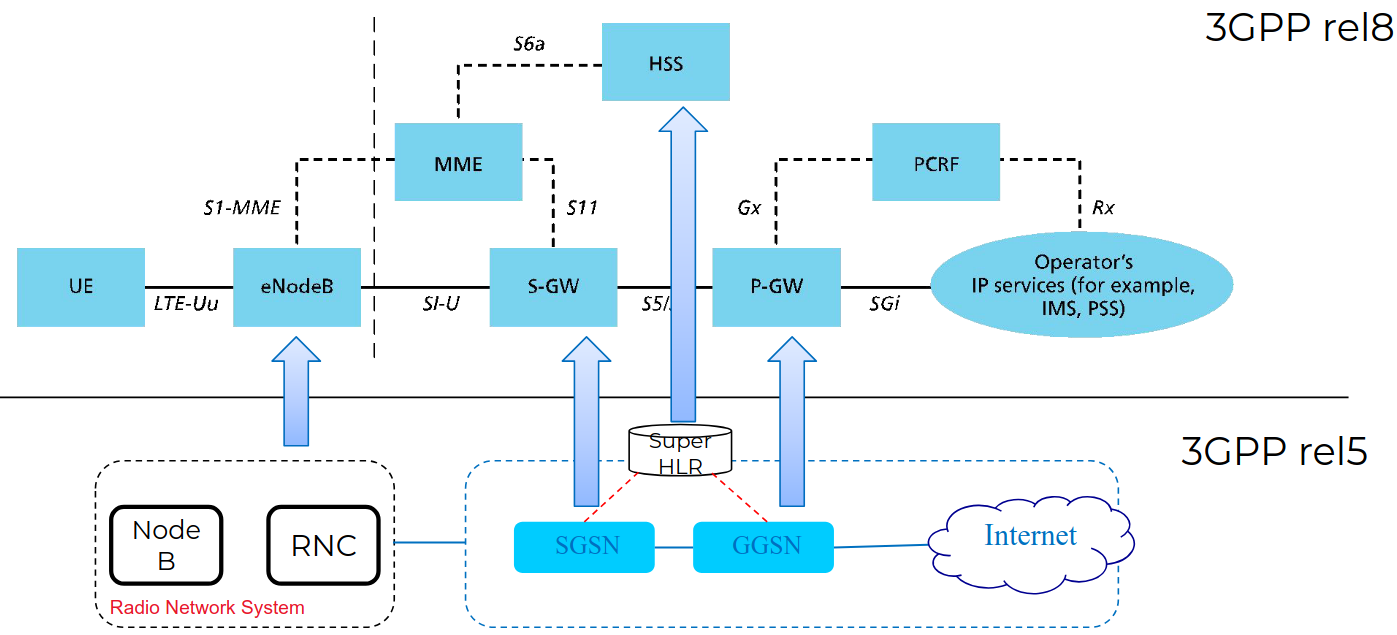
\includegraphics[width=0.95\linewidth]{img/mobile/3g4g}
\end{center}

Alcune differenze: 
\begin{center}
	\begin{tabular}{| m{3.5cm} | m{2cm} | m{2cm} |}
		\hline
		& 3G & 4G \\
		\hline
		Separazione logica di Control e Data plane &  No & Sì \\
		\hline
		Accesso multiplo  &WCDMA & OFDMA \\
		\hline
		Riuso frequenze & 100\% & 100\% flessibile \\
		\hline
		Larghezza banda & $5 MHz$ & $1.4$, $3$, $5$, $10$, $15$, $20 MHz$ \\
		\hline		
		Componenti rete accesso & NodeB e RNC & eNodeB \\
		\hline
		Handover & Soft e Hard & Hard \\
		\hline
		Trasporto & Circuito e Packet Switch & Packet Switch \\
		\hline
		Servizi voce e SMS & Interni alla rete & Esterni alla rete \\
		\hline
	\end{tabular}
\end{center}

Si introduce a livello architetturale una \textbf{separazione più netta} anche a livello logico \textbf{tra data e control plane}. Da NodeB (nome 3G per la Base Station) e RNC (Radio Network Controller, si occupa della gestione risorse radio) si ha solo il \textbf{eNodeB} (e sta per "\textit{evolved}"), questo è anche il motivo per cui l'handover è solo hard, non c'è più una RNC che può gestire multiple connessioni. Il dispositivo utente viene chiamato \textbf{User Equipment UE}.\\

La rete si divide in 
\begin{itemize}
	\item \textbf{E-UTRAN (Evolved Universal Terrestrial Radio Access Network)}, che comprende: 
	\begin{itemize}
		\item User Equipment UE
		\item eNodeB
	\end{itemize}
	\item \textbf{EPC (Evolved Packet Core)}, che contiene i moduli: 
	\begin{itemize}
		\item HSS Home Subscriber Server
		\item MME Mobility Management Entity
		\item P-GW Packet Data Network Gateway
		\item PCRF Policy Control and Charging Rules Function
		\item S-GW Serving Gateway
	\end{itemize}
\end{itemize}

\paragraph{Mobility Management Entity MME:} Si occupa di tutto ciò che è traffico di controllo e segnalazione all'interno della rete; il nodo di controllo responsabile del traffico di segnalazione tra Core Network (CN) e UE attraverso la suite di protocolli NAS (Non-Access Stratum). Tutto ciò che non è dati utente. Si occupa di: 
\begin{itemize}
	\item Gestione del contesto UE tramite operazioni NAS
	\item Gestione dei bearer (creazione, mantenimento, distruzione, \dots)
	\item Gestione della mobilità all'interno della Tracking Area (TA, insieme di BS)
	\item Gestione del paging
	\item Gestione dei aspetti di sicurezza e cifratura (genera e distribuisce chiavi, \dots)
\end{itemize}
Tra dispositivo utente e MME non transita mai traffico dati, solo controllo.\\

\newpage

\paragraph{Home Subscriber Server HSS:} Nodo che contiene le informazioni dell'utente, come: 
\begin{itemize}
	\item Profili Quality of Service QoS ammessi
	\item Eventuali restrizioni roaming
	\item Informazioni APN (Access Point Name)
	\item Identità dell'MME a cui UE è registrato
\end{itemize}

\paragraph{Packet Data Network Gateway P-GW:} Nodo al bordo tra rete LTE e reti esterne come Internet. Gestisce: 
\begin{itemize}
	\item Assegnamento dell'IP all'UE
	\item Garantisce QoS policy autorizzate da PCRF
	\item Filtro dei pacchetti IP downlink in bearer differenti per QoS
	\item Gestione della mobilità tra reti non-3GPP (CDMA-2000 o WiMAX)
\end{itemize}

\paragraph{Serving Gateway S-GW:} L'unico vero modulo solo data plane, nodo responsabile della gestione del traffico user-plane. Si occupa di:
\begin{itemize}
	\item Gestione di tutti i pacchetti IP degli utenti circolanti nella rete dell'operatore
	\item Funzioni di ancora mobile la gestione dei bearer quando UE è in fase di handover (dentro la tracking area)
	\item Funzionalità di buffering quando UE è in modalità IDLE-CONNECTED
\end{itemize}
Si tratta del punto di gestione, con un sottogruppo di eNodeB e, di conseguenza, utenti.\\

\paragraph{Policy Control and Charging Rules Function PCRF:} Svolge le funzioni di 
\begin{itemize}
	\item Controllo e autorizzazioni per singolo flusso a livello di P-GW
	\item Autorizza QoS secondo il profilo dell'utente (da HSS)
\end{itemize}
Contiene le "regole" da applicare all'utente, da negoziare e far applicare dal P-GW.\\

\paragraph{Evolved-NodeB eNodeB:} Primo all'interno di E-UTRAN; fornisce connettività radio all'UE e lo collega alla Core Network. Ha i compiti di una BS:
\begin{itemize}
	\item Gestione delle risorse radio
	\item Gestione dell'accesso multiplo di più UE
	\item Compressione degli header (utile per traffico VoIP)
	\item Connessione con S-GW e MME per traffico dati e controllo
	\item Informazioni sulla posizione degli UE
	\item Sicurezza e crittografia del canale radio
\end{itemize}
Prima di questo era tutto cablato, questa è la prima parte wireless.\\

\paragraph{Servizi operatore:} I servizi sono esterni alla rete: 
\begin{itemize}
	\item Chiamate: Voice over LTE (VoLTE): VoIP su rete LTE
	\item Internet
\end{itemize}

\subsubsection{Modulazione e Codifica Trasmissione}

Non verrà considerato, il Multiple Access, singolo utente. Con QPSK. Si ha una codifica digitale da tradurre in onde radio, a partire dai bit il processo di \textbf{trasmissione} è:
\begin{itemize}
	\item codifica dei bit in simboli tramite QPSK, 2 bit per simbolo
	\item modulazione usando una frequenza intermedia (IF); in LTE questa frequenza permette di variare leggermente la frequenza della portante (es: OFDMA lo usa per gestire più utenti)
	\item conversione in analogico (DAC)
	\item modulazione sulla portante: da banda base a banda traslata sulla portante
	\item selezione della componente in fase 
	\item trasmissione
\end{itemize}
\begin{center}
	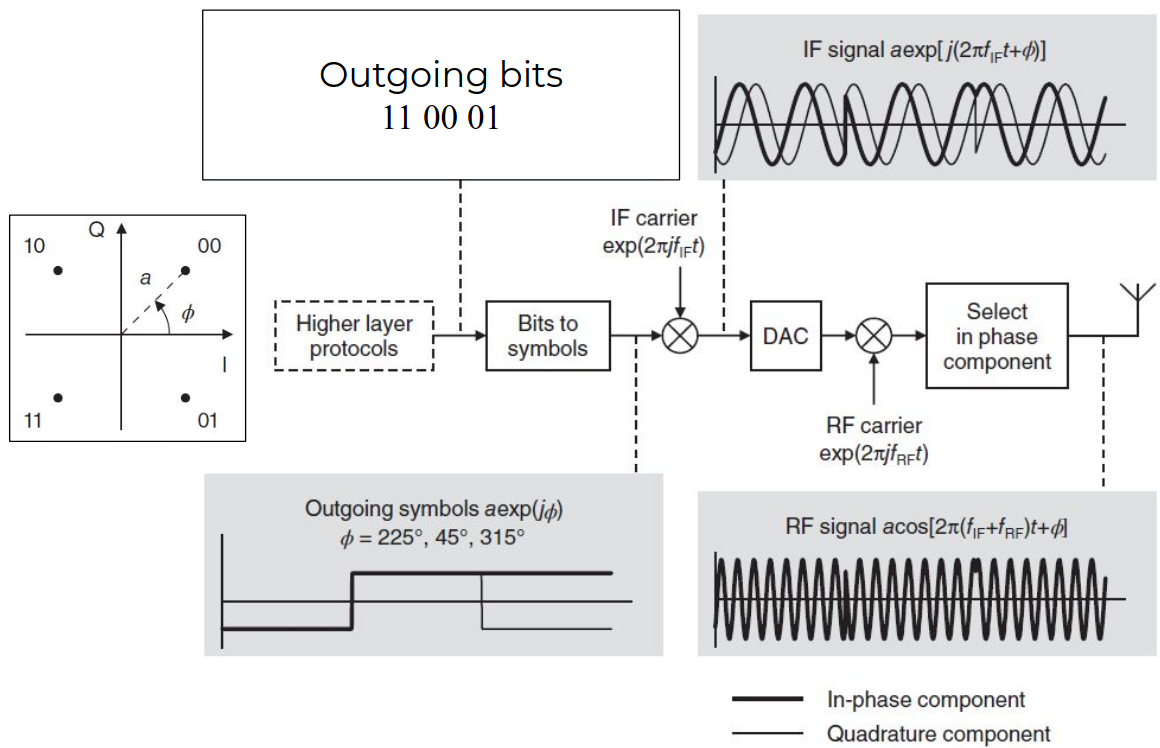
\includegraphics[width=0.9\linewidth]{img/mobile/mightbesending}
\end{center}

In \textbf{ricezione}: 
\begin{itemize}
	\item si misura sull'antenna il segnale, con relativo rumore e sfasamento indotto dalla mobilità ($\psi$)
	\item rimuovo la frequenza portante, torno in banda base
	\item filtro passa-basso per eliminare il rumore termico
	\item convertitore analogico digitale (ADC)
	\item Abbiamo trasmesso $\varphi$ e ricevuto $\varphi + \psi$ (sfasatura), per capire quanto è sfasato si fa channel estimation: stima dello sfasamento dovuto al canale (condizioni del canale), fatto tramite la ricezione di un pilot standard, per poi togliere quello sfasamento dall'onda dati ricevuta
	\item conversione da simboli a bit
\end{itemize}

Le \textbf{codifiche possibili} sono:
\begin{itemize}
	\item \textbf{BPSK Binary Phase Shift Keying}: usato solo per alcuni segnali di controllo a basso livello; non importa la qualità del canale, alcuni segnali di controllo fondamentali devono essere "compresi"
	\item \textbf{QPSK Quadrature Phase Shift Keying}: usato per tutti i messaggi radio di controllo e trasmissione dati in caso di scarsa qualità del segnale; permette un minore overhead di controllo, mantenendo una buona "comprensibilità" del segnale
	\item \textbf{16/64-QAM Quadrature Amplitude Modulation}: usato per la trasmissione dati
\end{itemize}

\paragraph{Scelta di modulazione e codifica:} Si ha un Adapting Modulation e Coding scheme: quantifica la qualità del canale in 4 bit e sceglie una modulazione:
\begin{center}
		\begin{tabular}{>{\centering\arraybackslash}m{0.8cm} >{\centering\arraybackslash}m{3cm} >{\centering\arraybackslash}m{3.5cm} >{\centering\arraybackslash}m{3.5cm}}
			\toprule
			\textbf{CQI} & \textbf{Modulation scheme} & \textbf{Coding rate (units of 1/1024)} & \textbf{Information bits per symbol} \\
			\midrule
			0  & n/a     & 0   & 0.00 \\
			1  & QPSK    & 78  & 0.15 \\
			2  & QPSK    & 120 & 0.23 \\
			3  & QPSK    & 193 & 0.38 \\
			4  & QPSK    & 308 & 0.60 \\
			5  & QPSK    & 449 & 0.88 \\
			6  & QPSK    & 602 & 1.18 \\
			7  & 16-QAM  & 378 & 1.48 \\
			8  & 16-QAM  & 490 & 1.91 \\
			9  & 16-QAM  & 616 & 2.41 \\
			10 & 64-QAM  & 466 & 2.73 \\
			11 & 64-QAM  & 567 & 3.32 \\
			12 & 64-QAM  & 666 & 3.90 \\
			13 & 64-QAM  & 772 & 4.52 \\
			14 & 64-QAM  & 873 & 5.12 \\
			15 & 64-QAM  & 948 & 5.55 \\
			\bottomrule
		\end{tabular}
\end{center}

Esempio: con CQI 7 si hanno 1.48 bit di informazione per ogni simbolo, quindi per 1024 bit 378 saaranno di informazione. Queste valgono per il data plane, il control plane ha una sua codifica molto meno variabile.\\

\newpage

\subsubsection{Riuso frequenze}
\begin{center}
	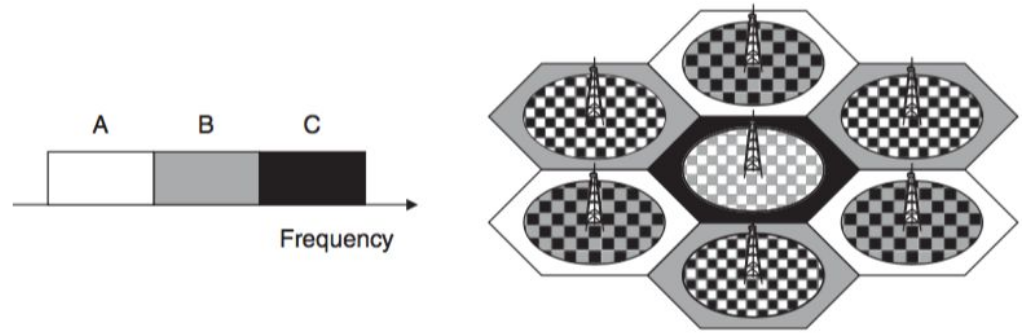
\includegraphics[width=0.9\linewidth]{img/mobile/riuso4g}
\end{center}
Utilizzo del 100\% delle frequenze disponibili come in UMTS.  Rispetto a UMTS la gestione delle interferenze è più semplice e coordinata tra le celle tramite l’apposita interfaccia X2. Le frequenze vengono coordinate ai bordi delle celle, in modo da usare una banda maggiore al centro, dove non possono esserci interferenze.\\

\subsubsection{Durata Simboli}

Non è casuale, si è decisa in base a
\begin{itemize}
	\item la distanza tra sottoportanti $15kHz$
	\item punti da campionare per la trasformata di Fourier $2048$
\end{itemize}

Di conseguenza
$$ T_S = \frac{1}{2048 \cdot 15000}s \approx 32.6 ns $$

Quindi il processore fisico deve avere una velocità adeguata. Un simbolo dura $2048 T_S = 66.7 \mu s$.\\

\newpage

\subsubsection{Struttura Slot}
I simboli sono organizzati in slot da $0.5ms$ ($15360 T_S$).\\

Si ha un cyclic prefix per evitare interferenza inter-simbolo causa del multipath. Per ogni slot ci sono 7 simboli ($66.7 \mu s$ ognuno), di cui $4.7$ o $5.2 \mu s$ sono di preambolo.
\begin{center}
	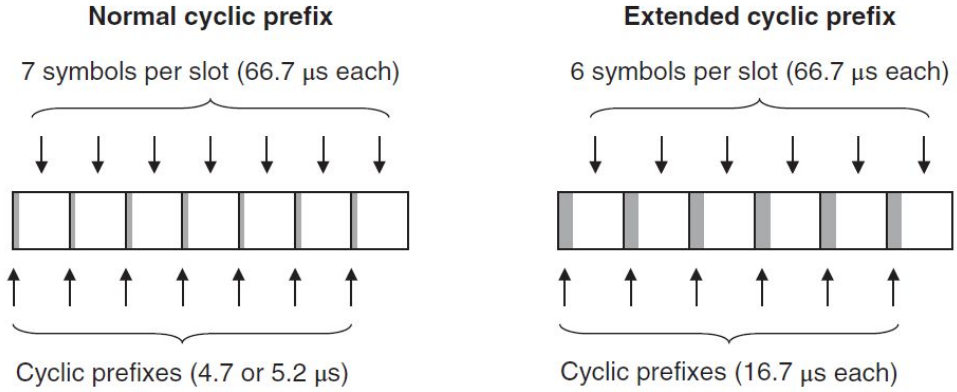
\includegraphics[width=0.7\linewidth]{img/mobile/cycprefix}
\end{center}

\subsubsection{Duplex}

Per la gestione del duplex, ogni eNodeB può essere configurato in 2 modalità comunicate a UE durante la fase di configurazione: 
\begin{itemize}
	\item \textbf{Frequency Division Duplex (FDD)}: Utilizzo di frequenze diverse per uplink e downlink
	\begin{center}
		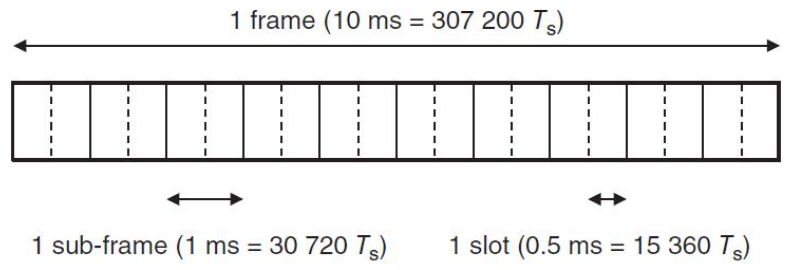
\includegraphics[width=0.5\linewidth]{img/mobile/fdd}
	\end{center}
	ogni frame di $10ms = 307200 T_S$ contiene 10 subframe/20 slot da $1/0.5ms$, quindi si hanno 140 simboli/frame (20x7) con normal cyclic prefix e 120 simboli/frame (20x6) con extended cyclic prefix.\\
	
	\newpage
	
	\item \textbf{Time Division Duplex (TDD)}: Utilizzo di una sola frequenza per uplink e downlink. Sono possibili 7 configurazioni:
	\begin{center}
		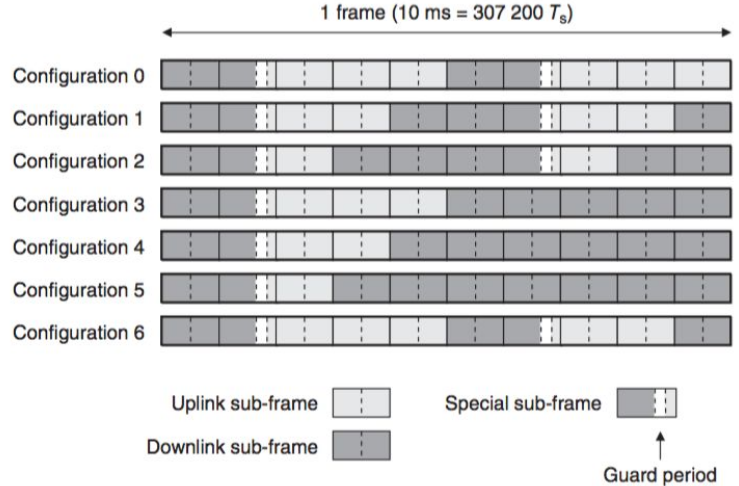
\includegraphics[width=0.7\linewidth]{img/mobile/tdd}
	\end{center}
	La configurazione è decisa in base all'utilizzo (se serve più downlink ne metto di più e viceversa).
\end{itemize}

\paragraph{Uplink Timing Advance:} Il guard period tiene conto dell'anticipo di trasmissione in uplink (Uplink Timing Advance). UE inizia a trasmettere in uplink in anticipo rispetto al tempo del frame della base station, altrimenti la ricezione avverrebbe in maniera disallineata dal tempo degli slot della BS, dato che dispositivi più lontani ci mettono più tempo a far arrivare il segnale. \\

Viene fornito un range di timing advance tra $0$ e $667\mu s$ per compensare la distanza. Per fare questo serve però che nessuno stia parlando in downlink durante il tempo di advance (altrimenti si avrebbe interferenza), per questo il guard time: serve a permettere l'advance per l'uplink senza interferenze.\\

\newpage

\subsubsection{Orthogonal Frequency Division Multiple Access OFDMA}

Gli eNodeB usano OFDMA: la banda viene divisa in piccole sotto-bande (sub-carriers) le cui frequenze non causano interferenze. LTE usa sotto-bande di ampiezza $15 kHz$ (frequenze intermedie IF di modulazione ortogonali). Più sotto-bande sono organizzate in \textbf{Resource Block} che rappresentano la minima quantità di risorse allocabili ad un singolo dispositivo.

\begin{center}
	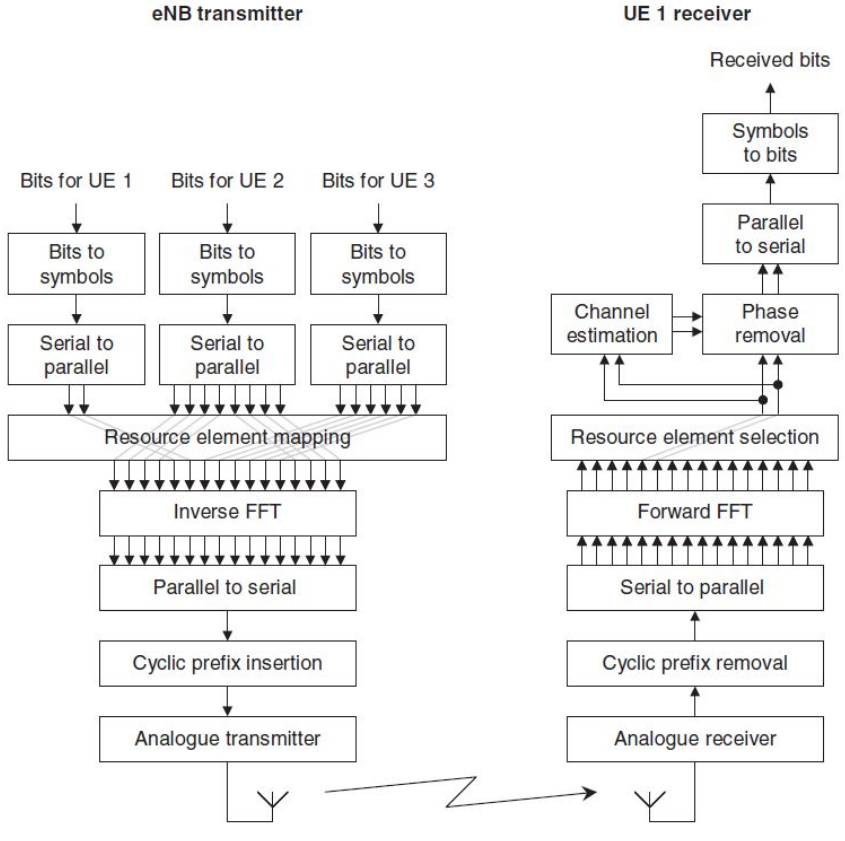
\includegraphics[width=0.75\linewidth]{img/mobile/utranofdma}
\end{center}

Gli step lato trasmettitore sono: 
\begin{itemize}
	\item Ogni flusso di bit distinto viene trasformato in simboli
	\item I simboli vengono mappati sulle risorse in frequenza (resource block allocati)
	\item Si applica la IFFT per trasformare i simboli mappati in frequenza nel dominio del tempo, ottenendo il segnale OFDM complesso
	\item I campioni temporali paralleli vengono ricombinati in un unico flusso seriale
	\item Si aggiunge il prefisso ciclico
	\item Il segnale viene convertito in analogico e trasmesso
\end{itemize}
Lato ricevitore bisogna fare il processo contrario, estraendo il flusso di bit per l'UE che sta ricevendo (sceglie di considerare solo i resource block a lui dedicati), correggendo il flusso dal rumore e sfasamento (tramite channel estimation).\\

Si hanno 12 sotto-bande di larghezza minima $180 kHz$ e 7 simboli in $0.5ms$. \\

\subsubsection{eNodeB Scheduler}
Tutte le comunicazioni da e per i dispositivi sono gestite dall'eNodeB. Lo scheduling ha risorse a disposizione (resource blocks) e determina come allocarli
\begin{center}
	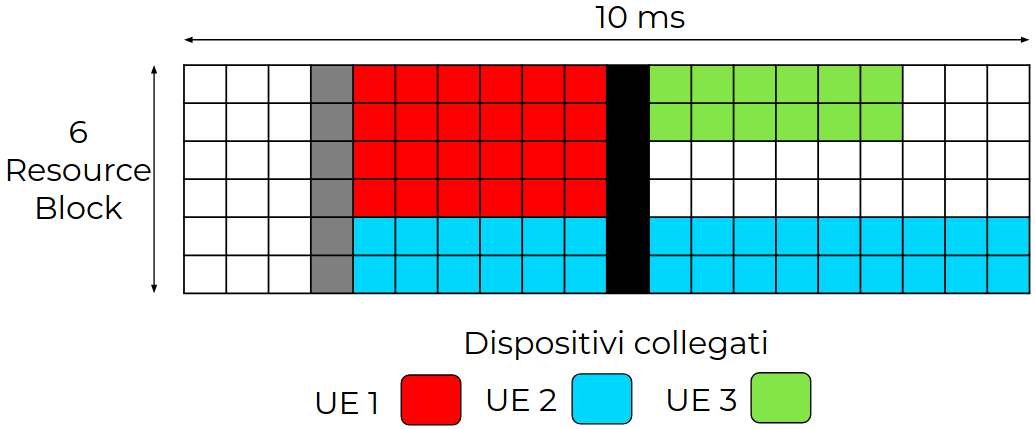
\includegraphics[width=0.75\linewidth]{img/mobile/alloc}
\end{center}
Blocchi grigi e neri sono dedicati alla trasmissione della BS. Tutto lo scheduling deve essere fatto real time (i.e., molto veloce).\\

\subsubsection{Velocità per UE}

Alla fine la banda disponibile per ogni singolo dispositivo dipende da molti fattori: 
\begin{itemize}
	\item Capacità del dispositivo (UE)
	\item Qualità del segnale radio: interferenze e distanza, determina la scelta della codifica
	\item Larghezza della banda in MHz: maggiore banda, maggior numero di resource block allocabili
	\item Configurazione TDD: a seconda della configurazione dell'eNodeB si possono avere differenti velocità di upload e download
	\item Numero dispositivi collegati
	\item Altri fattori non dipendenti dal canale radio: come congestione rete backhaul, congestione P-GW o altri fattori end-to-end
\end{itemize}

Le massime velocità teoriche per LTE Rel8 sono $300Mbps$ in download e $75Mbps$ in upload.\\

%End L17